For GASAL2 to work correctly, all data fields in the \texttt{gasal\_gpu\_storage\_t} structure must have their sizes specified at initialisation. This is problematic with BWA because sizes cannot be inferred beforehand. Even if we process a pack of 4000 sequences, each of them have an unpredictable number of chains. Furthermore, for each chain, the length of the query and target parts that have to be aligned are unknown too. We show a schematic view for this problem on Figure~\ref{fig:cpu-gpu-batches}. BWA processes query sequences by packs. On the picture, they are packs of 3 sequences (note the sequence numbers on the left). For each of them, they can have different number of seeds. The pack is split equally between sequences (this is difficult to show with a few number of sequences like here, but for example, a pack of 4000 sequences is split into 4 GPU batches of 1000 sequences each). All seeds extensions of a given sequence are processed in the same batch. Alignments of the same colour are processed in the same GPU batch. We can see that the total number of alignment is different depending on the number of chains, and each alignment has its own left and right lengths.

\begin{figure}[h!]
	\centering
	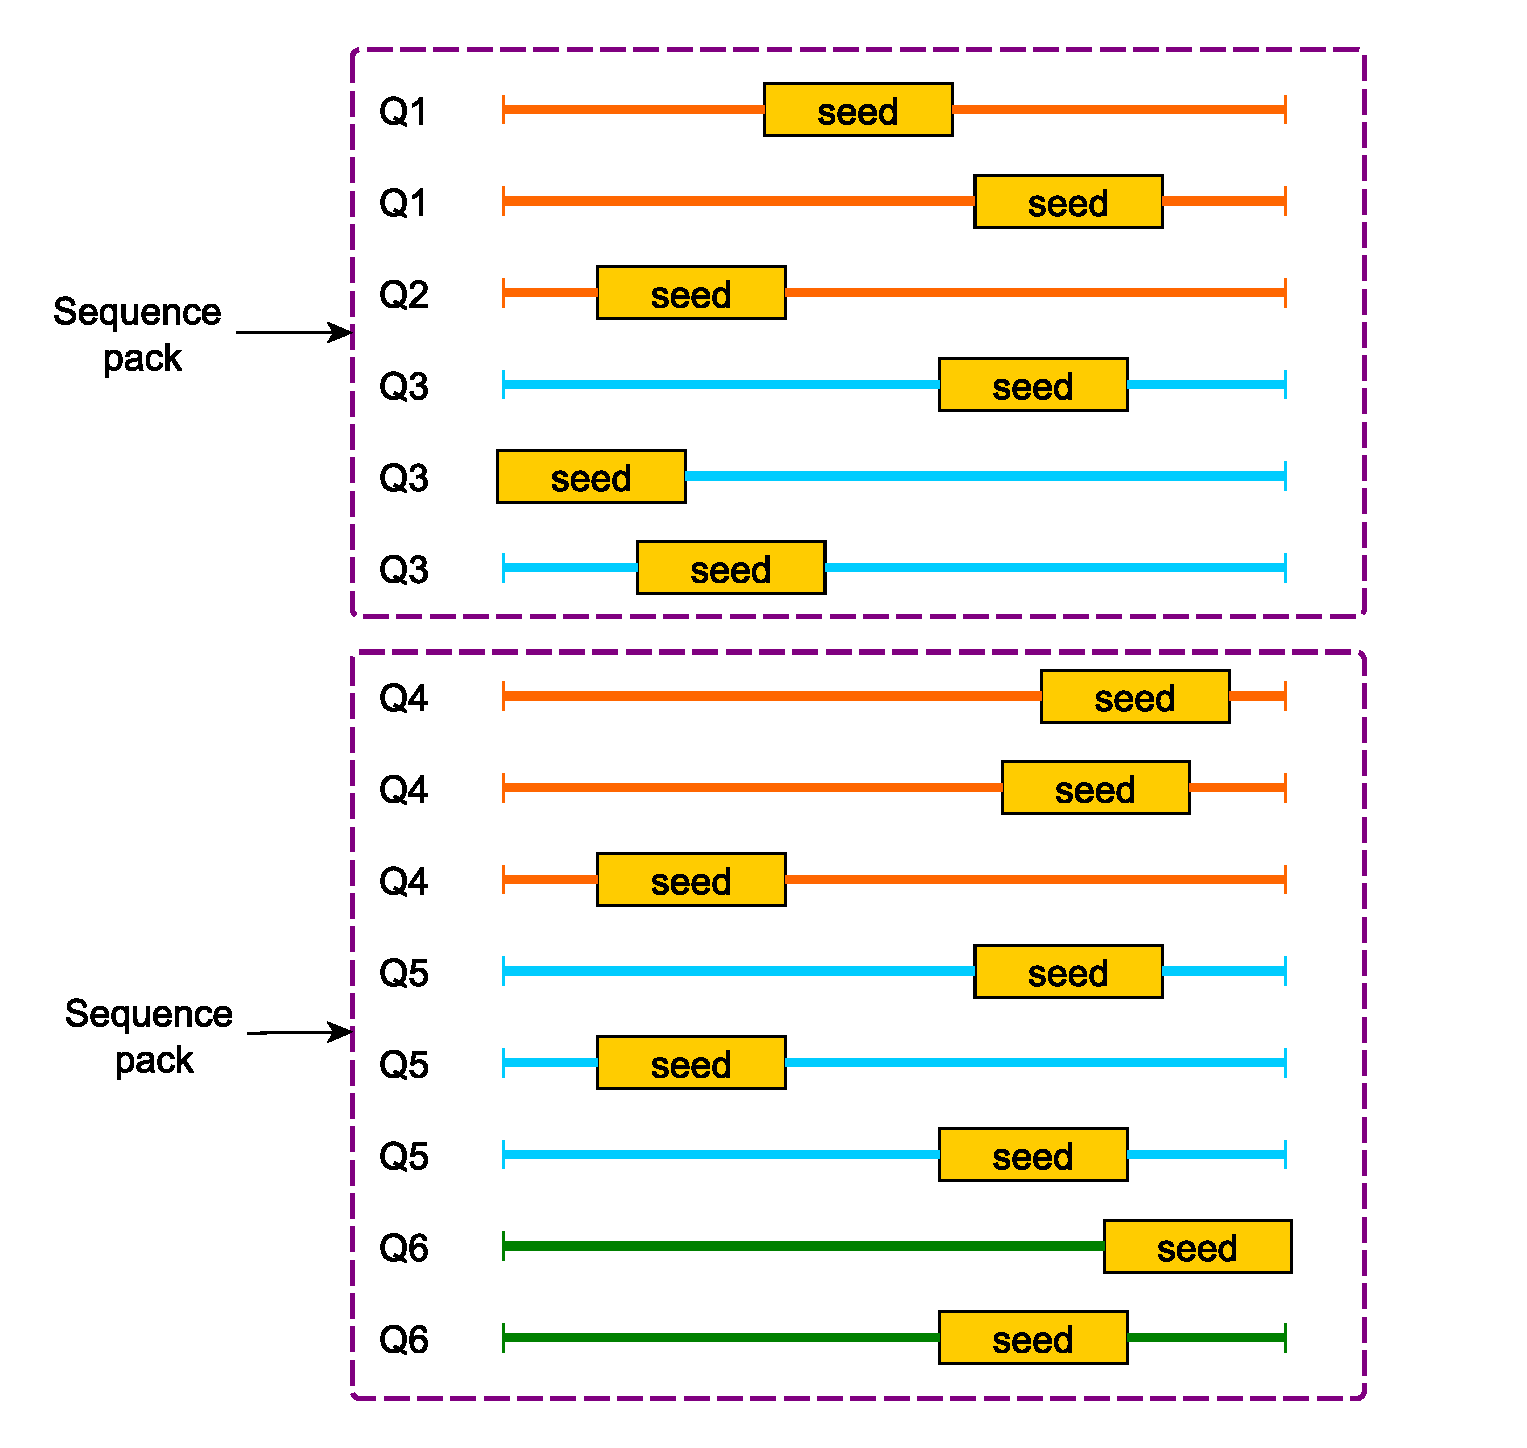
\includegraphics[width=1\linewidth]{cpu-gpu-batches}
	\caption{Representation of alignment distribution in sequences packs across GPU batches.}
	\label{fig:cpu-gpu-batches}
\end{figure}


We would need some automatic resizing whenever the size gets insufficient.
For a given data set, during testing phase, we can estimate a higher bound to allocate in the program source code. But this is not viable since we have to allocate much more memory than actually required.

In this section we will review the solutions we implemented. A simple approach was adopted for all the arrays carrying metadata for the sequences. We chose a more refined approach for the fields bearing the actual sequences to minimize overhead caused by reallocation.

\subsection{Memory reallocation for arrays fields}

A large number of fields in the \verb|gasal_gpu_storage_t| are containing information about the sequences entered. These fields are arrays of length equal to the number of sequences. As such, they do not store a very large amount of data, and their separation is clear (each slot of the array is holding information about one single sequence). For example, we need to store the length of each query and target, the offset of each each query and target, and so on. These fields are first allocated on host side, then they are copied onto the device, so they are allocated with \verb|CudaHostAlloc|. Since there are a lagre number of fields and they do not represent a major part of memory allocation, we decided to implement a simple realloc feature for all fields. This function is displayed on listing~\ref{lst:cudarealloc}. Note that on the \verb|gasal_gpu_storage_t| shown on Listing~\ref{lst:gpu_storage}, all fields do not have the same type: some are of type \verb|uint32_t|, others are \verb|uint8_t|, and so on. We made a simple use of C++ template to adapt this function to multiple types. It allocates a new memory area, copies the content of the former area, and frees it. It returns a pointer to the newly allocated area in memory filled with the previous data. This re-allocator is called by a larger function resizing all the necessary fields when the number of sequences filled exceeds the number of maximum sequences the structure can hold.

\begin{listing}[h!]
	\begin{minted}[frame=lines,
	framesep=2mm,
	baselinestretch=1.2,
	fontsize=\footnotesize,
	linenos,
	breaklines,
	frame=single]{C++}
// Function for general resizing
template <typename T>
T* cudaHostRealloc(void *source, int new_size, int old_size) 
{
	cudaError_t err;
	T* destination = NULL;
	if (new_size < old_size)
	{
		fprintf(stderr, "[GASAL ERROR] cudoHostRealloc: invalid sizes. New size < old size (%d < %d)", new_size, old_size);
		exit(EXIT_FAILURE);
	}
	CHECKCUDAERROR(cudaHostAlloc(&destination, new_size * sizeof(T), cudaHostAllocMapped));
	CHECKCUDAERROR(cudaMemcpy(destination, source, old_size * sizeof(T), cudaMemcpyHostToHost));
	CHECKCUDAERROR(cudaFreeHost(source));
	return destination;
};
	\end{minted}
	\caption{Reallocation function for CUDA allocated fields.}
	\label{lst:cudarealloc}
\end{listing}

With the progress currently made, the programmer in charge of integrating the library must take care of the sequence count and run the resizer when needed. Once the fields are reallocated to a bigger memory area, they keep their new size, so they don't need to be re-allocated until the next time the new maximum capacity is exceeded. The structure can store the current number of sequences filled into it, and the maximum number. 

We chose a different approach for the actual sequences because of their much more important size, making them much longer to reallocate.

\subsection{Extensible data structure for sequences}

Using the same reallocation for the sequences could have been possible, but unpractical. In fact, these memory allocations and frees are costly in time. While this is reasonable for smaller arrays having only 4-bytes elements (like \verb|uint32_t|), it takes too much time with the sequences arrays. The query and target fields are storing all the DNA strings butted together (one field for all queries, the other for all targets). In terms of space taken, on BWA, if a pack of 1000 sequences is processed in a GPU batch, it can require between 10 000 to even 100 000 chains, making it up to 200 000 alignments to proceed (most chains needing both left and right extension). Each base being stored on one byte, it makes these fields 20 to 30 times bigger than the others.

For this issue, we designed a structure of linked list to allocate more and more memory progressively without needing to move around already existing data. This structure shown on Listing~\ref{lst:extensiblehostbatch} starts with a single element and each of them carries some metadata about its content size to ensure correct filling. It stores:

\begin{itemize}
	\item the sequences, butted together, in the field \verb|*data|,
	\item how many bytes are already stored, in field \verb|data_size|,
	\item the total size available in bytes, in the field \verb|page_size|,
	\item the data \verb|offset|, which is equal to the data size of the previous element of the linked list,
	\item A flag telling is the structure can store new data or not, \verb|is_locked|, set to 0 or 1,
	\item and of course, as for all linked list, a pointer to the next element.
\end{itemize}

\begin{listing}[h!]
	\begin{minted}[frame=lines,
	framesep=2mm,
	baselinestretch=1.2,
	fontsize=\footnotesize,
	linenos,
	breaklines,
	frame=single]{C++}
struct host_batch{
	uint8_t *data;
	uint32_t page_size;
	uint32_t data_size;
	uint32_t offset;
	int is_locked;
	struct host_batch* next;
};
typedef struct host_batch host_batch_t;
	\end{minted}
\caption{The linked list structure for sequences on host.}
\label{lst:extensiblehostbatch}
\end{listing}

The sequences are filled by a dedicated function from GASAL2 that takes care of allocating more memory if needed. This function takes as input the sequence to add, the storage structure, and if it is a query or target sequence to fill, and operates with the algorithm shown on Algorithm~\ref{algo:extensiblefunction}. We represent the fields belonging to an element with the symbol $\rhd$, like the symbol \verb|->| is used in C++ to get the field belonging to a pointer to a structure.


\begin{algorithm}[h!]
	\caption{Behaviour of the sequence filler function}
	\label{algo:extensiblefunction}
	\begin{algorithmic}[1] % The number tells where the line numbering should start
		\Function{Fills one sequence in an linked list }{$gasal\_gpu\_storage\_t$, $seq$, $seq_length$, $seq_offset$, $data\_source$}
		
		\State Select query or target linked list from $data\_source$
		\State Select first non-locked linked-list element, $~e$
		\State Compute padding length $padding\_length$
		\State $total\_length \leftarrow padding\_length + seq\_length$
		
		\If{$e$ is the last element \textbf{and} $total\_length \geqslant e\rhd page\_size - e\rhd data\_size$}
			\State Create new element twice as big
			\State Append it to the last element $e$
			\State Select last element (newly added) of the linked list, define it as $e$
		\EndIf
		
		\If{$e$ is not the last element \textbf{and} $total\_length \geqslant e\rhd page\_size - e\rhd data\_size$}
			\State $e\rhd next\rhd offset \leftarrow e\rhd offset + e\rhd data\_size $
			\State Mark $e$ as locked
			\State Select next element $e\rhd next$ of the linked list, define it as $e$
		\EndIf
		
		%\If{$total\_length \leqslant e\rhd page\_size - e\rhd data\_size$}
			\State Store the sequence in $e\rhd data$ add the padding
			\State $e\rhd data\_size \leftarrow e\rhd data\_size + total\_size$
		%\EndIf
		
		
		\Return $offset$
		\EndFunction
		
	\end{algorithmic}
\end{algorithm}

In the beginning, the first non-locked element is selected. Then the algorithm operates in three main steps. 

\begin{enumerate}
	\item First (line 6), it checks if the selected element is the end of the chain, and if there is not enough space in it. If so, the only solution is to create a new element to append at the end of the chain.
	\item Then (line 11), it checks if there is more elements down the chain, but if the current element is full. This happens when the chain has been creating new elements during previous fillings and kernel launches. We already selected the first non-locked element, so if it is full, we simply jumps to the next one, and lock the previous one so that we don't try to fill it anymore.
	\item At this point (line 16), we have reached an element who must have enough free space for the sequence (either by having an element available from the beginning, or we filled the current available one so we locked it and moved to the next one, or we created a new one), so we fill it with the sequence and its offset.
\end{enumerate}

In the end, the function returns the current offset, corresponding to the number of bytes totally present in the linked list, which is needed to continue the filling for the next sequence.

Globally, we have a linked list of structures filled by full sequences. In other words, for the sake of not splitting the sequences between two elements, we do not exactly fill each element up to its maximum capacity. 

When copying the batches onto the device, all elements are processed using \verb|CudaMemCpy|. The size to copy is directly given by the field \verb|data_size|. At this moment, all the elements in the linked list are set as "non-locked". This way, they can be re-used for future launches. The linked list can only grow in size, and always grows ever bigger to minimize the possibility of having to do another allocation later on. This is why we implemented this "locked" flag to get the information if the element has been filled for the current batch, to know where to start filling up.

All in all, this allocation scheme allows to get more memory space without moving around already existing data, always re-use all the previously created memory chunks in the linked list, and creates bigger and bigger elements to lower the probability of having to allocate a high number of them.

%\vspace{0.1\textheight}
\section*{Wrap-up}
In this chapter, we reviewed all the modifications and new implementation we carried out to successfully integrate GASAL2 in BWA. We started from a demonstrator already presenting the processing in pack of sequences, and we first ported it to C++ to run it with the newer version of GASAL2. We created a CUDA kernel that replicates the behaviour of the original C function in BWA. We integrated the library with our "seed-only" paradigm to tackle the issue of processing both sides of the extension at the same time, which created its own issues with score synchronisation between left and right sides, that we addressed. The memory management is now done with a reallocation in number of alignments, along with a linked list of elements for the actual data to minimize the number of memory operations. Finally, we tested this implementation in our hardware with a sample data set, that we will present in the next chapter.


